\documentclass[12pt]{article}
\usepackage{amssymb}
\usepackage{amsmath}
\usepackage{amsthm}
\usepackage{array}
\usepackage{graphicx}
  \DeclareGraphicsRule{*}{mps}{*}{}
%\usepackage{bbm}
\usepackage{marvosym}
\usepackage{enumerate}
\usepackage{txfonts}
\usepackage{paralist}
\usepackage{pdfpages}
\usepackage{multicol}
\usepackage{pgfplots}
\pgfplotsset{compat=1.5}
\everymath{\displaystyle}

%\usepackage{showframe}

\pagestyle{empty}

\usepackage{fullpage}
%% \addtolength{\hoffset}{-1.5cm}
%% \addtolength{\textwidth}{3cm}

%% \addtolength{\voffset}{-1.5cm}
%% \addtolength{\textheight}{3cm}

\setdefaultleftmargin{0pt}{}{}{}{}{}

\newcommand{\vv}[2]{#1}

\hyphenpenalty=5000
\tolerance=1000
\setlength{\parindent}{0pt}

\begin{document}

\thispagestyle{empty}
\begin{center}
  \textbf{ MATH 202 -- Slope fields 
  --- Spring 2026
    }
\end{center}

Consider the differential equation $\frac{dy}{dx} = -\frac{x}{y}.$
\begin{enumerate}[a.]
\item I've marked one of the corner points of the grid below. What are the coordinates at that point? 
\item Plug the coordinates at that point into the differential equation to get out a slope. \\
(Hint: The answer is $-2$. Why?)
\item Draw a little tiny tangent line at that point with the slope you got from part b.
\item Repeat this process at each of the grid points below,
and draw small lines at each point with the slope you find.
(You don't need to officially evaluate the differential equation at every
one of these points, because there are a lot of them, but do enough
that the pattern becomes clear.)
\begin{center}
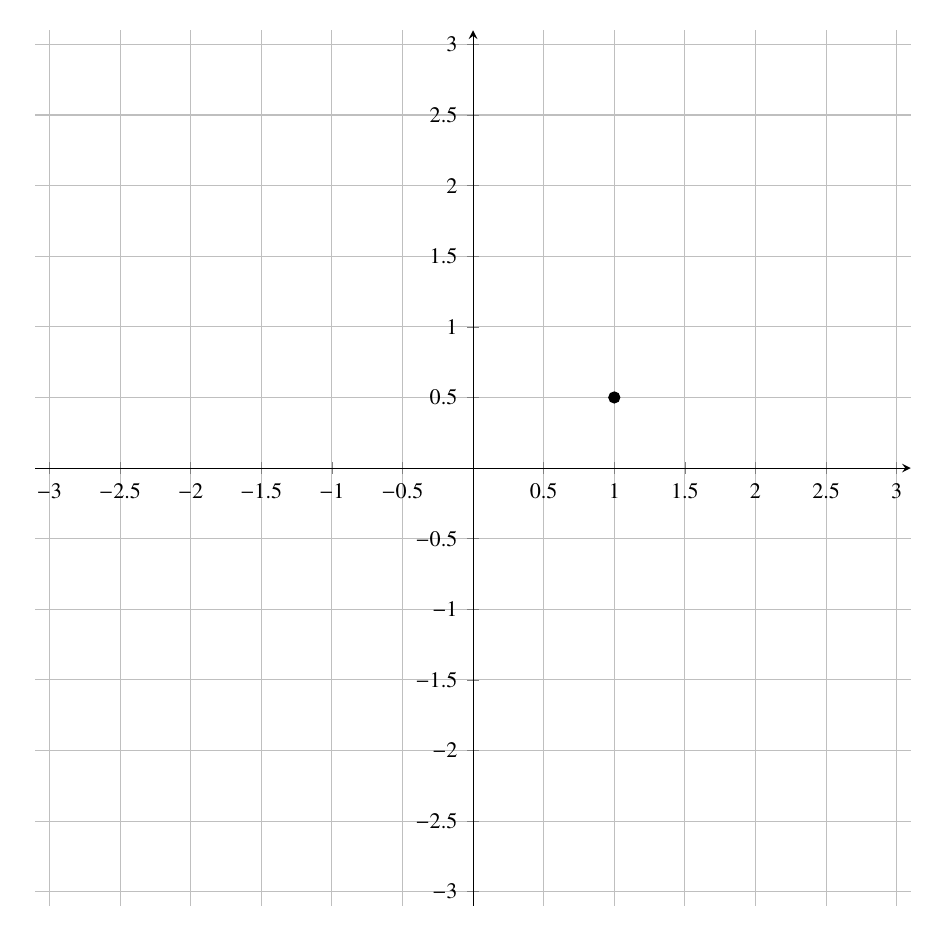
\begin{tikzpicture}
	\begin{axis}[width=5in, height=5in,
		grid=major,
		tick label style={font=\footnotesize},
		%xtick={-3,...,3},
		%ytick = {-3,...,3},
		xmin = -3.1, xmax = 3.1,
		ymin = -3.1, ymax = 3.1,
		axis x line = middle,
		axis y line = middle,
		grid=both,
		]
    \addplot[mark=*] coordinates{(1,0.5)};
	\end{axis}
\end{tikzpicture}
\end{center}
\item Pick several different initial conditions, and follow the slope field 
you've generated to sketch the solution curves that result. What do you think
the solutions to this differential equation are?
\end{enumerate}

\end{document}
